\section{System Performance}{\label{secSysperf}}
  
Handover means that the system will have passed the NSF and DOE Construction Completeness Review \#3 (CCR3).  Noting the formal close out of the MREFC grant and AURA cooperative agreement occurs with CCR4. The as delivered system will be {\it capable} of delivering images that satisfy the construction design requirements derived from the Science Requirements Document (SRD: \cite{LPM-17}).  These requirements are defined in the LSST System Requirements (LSR: \cite{LSE-29}) and Observatory System Specifications (OSS: \cite{LSE-30}) documents. Following the final phase of commissioning which includes science validation (SV) observations, the state of the system will be assessed and the readiness assessment of the system and team to begin the survey will be made. Further optimization by the Operations team will be planned to ensure the system operates {\it reliably} at the needed level of performance capabilities. 

Rubin has developed a high level set of metrics summarizing the system performance with respect to overall survey efficiency. We need to simultaneously ensure that both 1) the system is producing viable science quality images and data products and 2) that the observing and acquisition of this data is efficient.  To this end, we gauge the overall system survey capabilities in a 2--parameter space shown in Figure~\ref{fE}, marking the system $+$ atmospheric contribution to delivered image quality versus the dimensionless survey efficiency or speed, {\it fE} -- integrated Normalized \'{E}tendue.  The combined summary Normalized \'{E}tendue metric ({\it fE}) is the product of 4 unitless {\it f-metrics} that gauge system contributions to the ''survey speed'', these are: 1) { \it fS -- System Sensitivity} captures overall efficiency of recording photons from the sky and is driven by optical transmission, sensor quantum efficiency, sky brightness and image quality; 2) {\it fA - Fill Factor} captures the recorded area of the focal plane array relative to the area delivered by the optical system; 3) {\it fO - Observing Efficiency} captures the efficiency with which available observing time is scheduled and utilized for survey observations and 4) {\it SA - System Availability} a final factor that captures overall operational efficiency that takes into account weather and observatory downtime.   If the system is producing appropriate image quality and the system and team are acquiring data efficiently, we can confidently start the LSST.  The ''start'' criteria quantify the threshold in the 2-parameter performance space that is needed to achieve this goal.

\begin{figure}%[!ht]
\centering
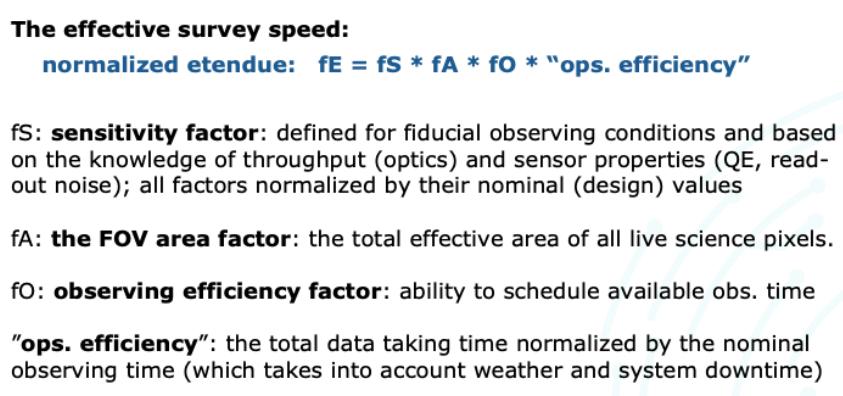
\includegraphics[width=0.75\linewidth]{fE.png}
\caption{Dimensionless survey efficiency factor, fE. System Availability is the most uncertain at this time. The current state of each factor is discussed below and the quantitative criteria for starting the LSST with respect to each factor is assessed.}
\label{fE}
\end{figure}

These {\it f--factors} are defined to be dimensionless and normalized by the corresponding SRD derived design values. They can be traded against each other as time gained or lost.  For example, deterioration in the mirror reflectivity can be easily translated to factor fS, and traded against time (e.g. time lost to recoating, the system efficiency), or against loss of sensor area (fA).
The key point is that it is possible to define a simple measurable quantity (fE) that is an excellent numerical approximation for LSST science goals. Thus, we can think of the effective speed of executing the LSST (in units of the nominal speed) in terms of recognizable elements:  fE $=$ effective area $\times$ effective FOV $\times$ cadence $\times$ 1-downtime.

In Figure~\ref{speed}, we show the state of our understanding of the image quality and survey speed before we went on sky with LSSTCam. The white circle is a forecast based on expectations before we went on sky with some as built elements of the system accounted for. We believe there is nothing limiting us reaching that circle, but the current performance is not there yet. 

\begin{figure}[t]
\centering
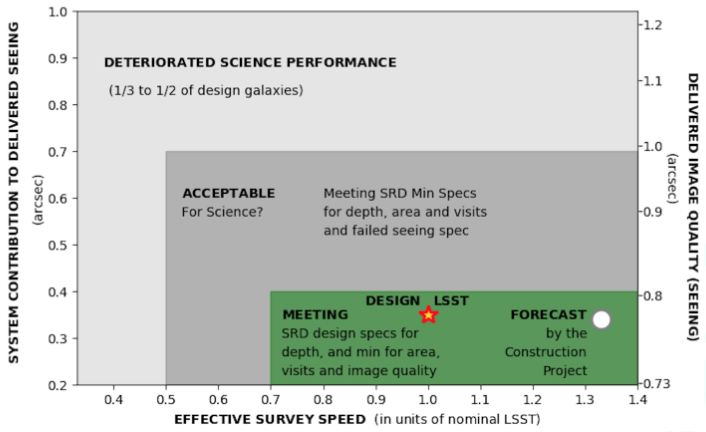
\includegraphics[width=0.85\linewidth]{speed.png}
\caption{Image quality versus effective survey speed, fE. The system contribution to the delivered image quality (sDIQ) is shown on the left vertical axis and the delivered image quality including the atmosphere (added in quadrature) is on the right. The LSST specifications are  accomplished with nominal speed fE = 1.0 and sDIQ = 0.4$\arcsec$ in this diagram. Current performance is assessed below. The white circle is representative of where we want to drive the performance, but we have not reached it yet.}
\label{speed}
\end{figure}

There are three regions defined in the diagram, green, light grey and dark grey, representing broad levels of operational performance towards meeting the 10--year LSST objectives. Clearly we want to be in the green shaded region and to the lower right in that space. The boundaries of the green box are defined by the minimum design specification from the SRD (upper) and stretch goals (lower) for the system image quality contribution.  The light gray space is unacceptable for science and the dark gray space covers the area where SRD minimum specifications are met for depth, area of LSST, and visits, but fails to meet the specification for system contribution to the DIQ (0.4$\arcsec$). 

As of CCR2/ORR1, the current values for the f factors are given in Table~\ref{tab:factors}. For fA, the value is set by the number of science pixels available (each with 0.2 $\times$ 0.2 arcsec$^2$ on the sky). Accounting for the active pixels meeting specifications, the factor is fully 99$\%$. The fS factor includes read noise, QE, vignetting, optical throughput (filter, lens transmission, mirror reflectance) and DIQ (so DIQ affects both axes in our diagram). The observing efficiency factor, fO, is a function of how many visits of the right exposure time can be observed given telescope performance (how fast we move and settle). Finally, system availability is defined as the open shutter science time compared to the total elapsed time working on the on--sky programs. Presently, if we consider only times when we are in the science data taking mode (doing LSST like observations) we have sustained 85$\%$ availability over a week long period. If we consider other system tuning in the denominator mixed with the science SV observations, the availability is about 75$\%$. 

The range of performance between what has been achieved over periods of SV and the best performance is shown in Figure~\ref{speed2}. The goal of further optimization is to use the available technical "knobs" to tune the performance and make it more reliable. Some of the knobs are to be deployed in the September -- October 2025 shutdown. The knobs are, at a high level, a laser alignment system, the active optics system (AOS) and associated wavefront sensing/analysis, thermal control of the M1M3 cell, thermal control of the top end assembly (volume around M2), and the dome ventilation (active control of louvers and installation of the air distribution ducting, both not yet deployed). Deployed or not, all of these are under active work and progress has been made on a number of fronts not yet reflected in Figure~\ref{speed2}. Mainly, but not entirely,  because the time available on sky has been limited since CCR2/ORR1. 

\begin{table}[]
\renewcommand{\arraystretch}{2}
\small
\centering
\caption{Current f factor status}\label{tab:factors}
\begin{tabular}{cccc}
\hline
factor & Description& SV Sustained Performance & Needed to Start LSST \\
\hline \hline
DIQ & System Contribution (PSF FWHM)  & 0.6$\arcsec$ & 0.45$\arcsec$ \\
fA & FoV area factor & 0.99 & 0.99 \\
fS & Sensitivity factor & 0.94 & 1.30 \\
fO & Observing Efficiency & 0.97 & 1.05 \\
SA & System Availability (up and taking data) & 0.75 & 0.75 \\
fE & Normalized \'{E}tendue & 0.68 & 1.01 \\

\hline
\end{tabular}
\end{table}

\begin{figure}[t]
  \centering
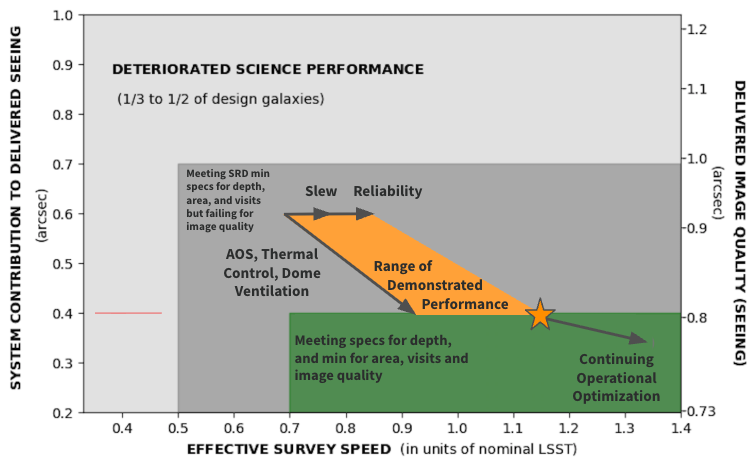
\includegraphics[width=0.85\linewidth]{speed2.png}
\caption{Image quality versus effective survey speed, fE with performance presented at CCR2-ORR1. Upper left of the orange performance region is sustained over week long periods in SV. The best performance (capability) is represented by the lower right vertex of the region. We are focused on getting reliable performance there and beyond as indicated. The minimum performance needed to begin the LSST is discussed below.}
\label{speed2}
\end{figure}

The current capability and reliability of the system as described in Table~\ref{tab:factors} and Figure~\ref{speed2} form the basis of optimization criteria described in the next section that the Operations team will use to gate starting the LSST. 

\newpage


